\newcommand{\x}{$\times$}

\newcommand{\figBootstrapping}{
    \begin{figure}[t]
        \begin{center}
            \includegraphics[width=0.65\columnwidth]{figures/ag_bootstrapping.pdf}
            \caption{Multiplicative budget over time. Bootstrapping can be used to reset a ciphertext's multiplicative budget.}
            \label{fig:bootstrapping}
        \end{center}
    \end{figure}
}

\newcommand{\figKScompare}{
  \begin{figure}[t]
    \begin{center}
        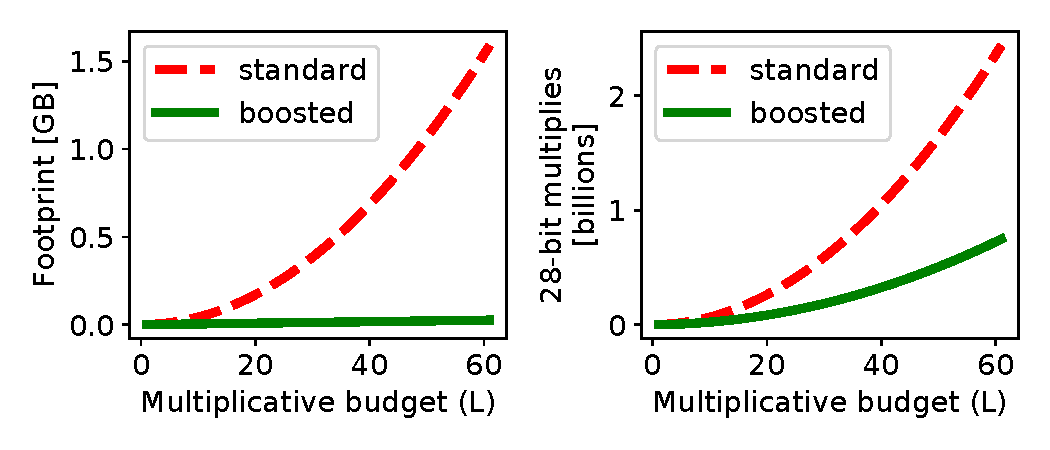
\includegraphics[width=0.75\columnwidth]{plots/ks_comparison.pdf}
	\caption{Comparison of footprint and compute for standard and boosted keyswitching.}
        \label{fig:ksCompare}
    \end{center}
  \end{figure}
}

\newcommand{\figBootstrappingFrequency}{
  \begin{figure}[t]
    \begin{center}
        \includegraphics[width=0.85\columnwidth]{figures/ag_bootstrappingFrequency.pdf}
        \caption{Computation cost as a function of max ciphertext size for narrow (left) and wide (right) deep FHE programs.}
        \label{fig:bootstrappingFrequency}
    \end{center}
  \end{figure}
}

\newcommand{\tblOpBalance}{
    \begin{table}[t]
            \begin{footnotesize}
        \begin{center}
            \begin{footnotesize}
            \begin{tabular}{lrclr}
                \toprule
                         & \multicolumn{3}{c}{\textbf{Boosted keyswitching}} & \textbf{Standard} \\
                Ops      & changeRNSBase  & + & other &  \textbf{keyswitching}\\
                % alex: Changed the numbers to reflect only keyswitching; not
                %       full homomorphic multiply. This is a homomorphic rotate
                %       minus one add.
                % alex: Technically, the L^2 Add terms in both boosted and
                %       standard should be L(L-1) as it takes L-1 additions to
                %       sum up L numbers. But, we probably don't care...
                \midrule
                Mult     & $3L^2$  & + & $4L$    & $2L^2$ \\
                Add      & $3L^2$  & + & $2L$    & $2L^2$ \\
                NTT      &         &   & $6L$    & $L^2$ \\
                \midrule
                % alex: I don't think it N=64K is necessary as N doesn't appear
                %       anywhere in the formulas. Alternatively, we should
                %       multiply everything by N.
                %\multicolumn{3}{l}{At $N$=64K, $L$=64:} \\
                \multicolumn{3}{l}{At $L$=60:} \\
                \midrule
                Mult     & 10,800 & + & 240         & 7,200 \\
                Add      & 10,800 & + & 120         & 7,200 \\
                NTT      &        &   & 360         & 3,600 \\
                \bottomrule
            \end{tabular}
            \end{footnotesize}
        \end{center}
            \end{footnotesize}
            \caption{Operation breakdown for boosted vs.\ standard keyswitching as a function of multiplicative budget ($L$), and for $L$=60. Boosted keyswitching operations are split by whether they happen within or outside \texttt{changeRNSBase()}.}
        \label{tbl:opBalance}
    \end{table}
}

\newcommand{\figPipeline}{
    \begin{figure}[t]
        \begin{center}
            \includegraphics[width=\columnwidth]{figures/ag_pipeline.pdf}
            \caption{Illustration of how vector chaining is used for part of a homomorphic multiply.}
            \label{fig:pipeline}
        \end{center}
    \end{figure}
}

\newcommand{\figInterClusterTiling}{
    \begin{figure}[t]
        \begin{center}
            \includegraphics[width=0.7\columnwidth]{figures/ag_interClusterTiling.pdf}
            \caption{Transposing a 16-element vector across two lane groups.}
            \label{fig:interClusterTiling}
        \end{center}
    \end{figure}
}

\begin{comment}
\newcommand{\tblParams}{
    \begin{table}[t]
        \begin{center}
            \begin{tabular}{ll}
                \toprule
                Parameter &Definition \\
                \midrule
                $N$ &Degree of ciphertext polynomials \\
                $Q$ &Modulus of ciphertext polynomial coefficients \\
                \bottomrule
            \end{tabular}
        \end{center}
        \caption{FHE parameters and their definitions.}
        \label{tbl:params}
    \end{table}
}
\end{comment}

\newcommand{\tblUtilization}{
\begin{figure}[t]
    \centering
    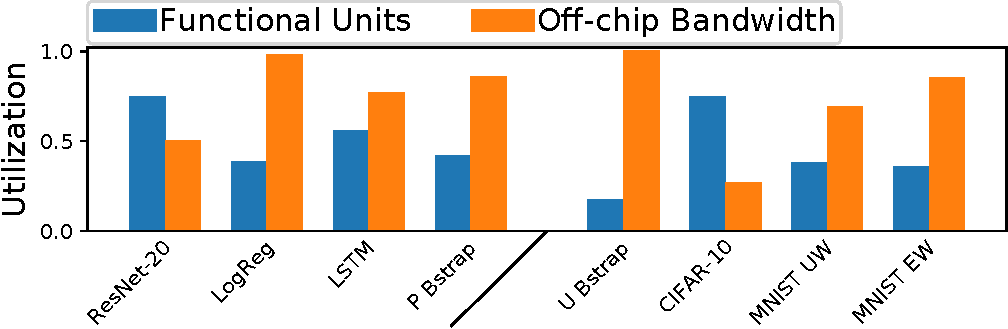
\includegraphics[width=0.7\columnwidth]{plots/utils.pdf}
    \caption{Functional unit and memory bandwidth utilization.}
    \label{tbl:utilization}
\end{figure}
}

\newcommand{\figNewKS}{
    \begin{figure}[t]
        \begin{center}
            \includegraphics[width=\columnwidth]{figures/ag_newKS.pdf}
            \caption{New keyswitching implementation.}
            \label{lst:newKeyswitching}
        \end{center}
    \end{figure}
}

\newcommand{\figWorkflow}{
  \begin{figure}[t]
    \begin{center}
        \includegraphics[width=0.65\columnwidth]{figures/ag_workflow.pdf}
        \caption{FHE can offload computation to the cloud securely.}
        \label{fig:workflow}
    \end{center}
  \end{figure}
}
\newcommand{\figCRB}{
  \setlength{\columnsep}{7pt}
  \begin{figure}[t]
      \begin{center}
      \includegraphics[width=0.6\columnwidth]{figures/ag_crb.pdf}
      \caption{Microarchitecture of the change RNS base (CRB) unit.}
      \label{fig:crb}
    \end{center}
  \end{figure}
}

\newcommand{\figOverview}{
  \begin{figure}[t]
    \begin{center}
        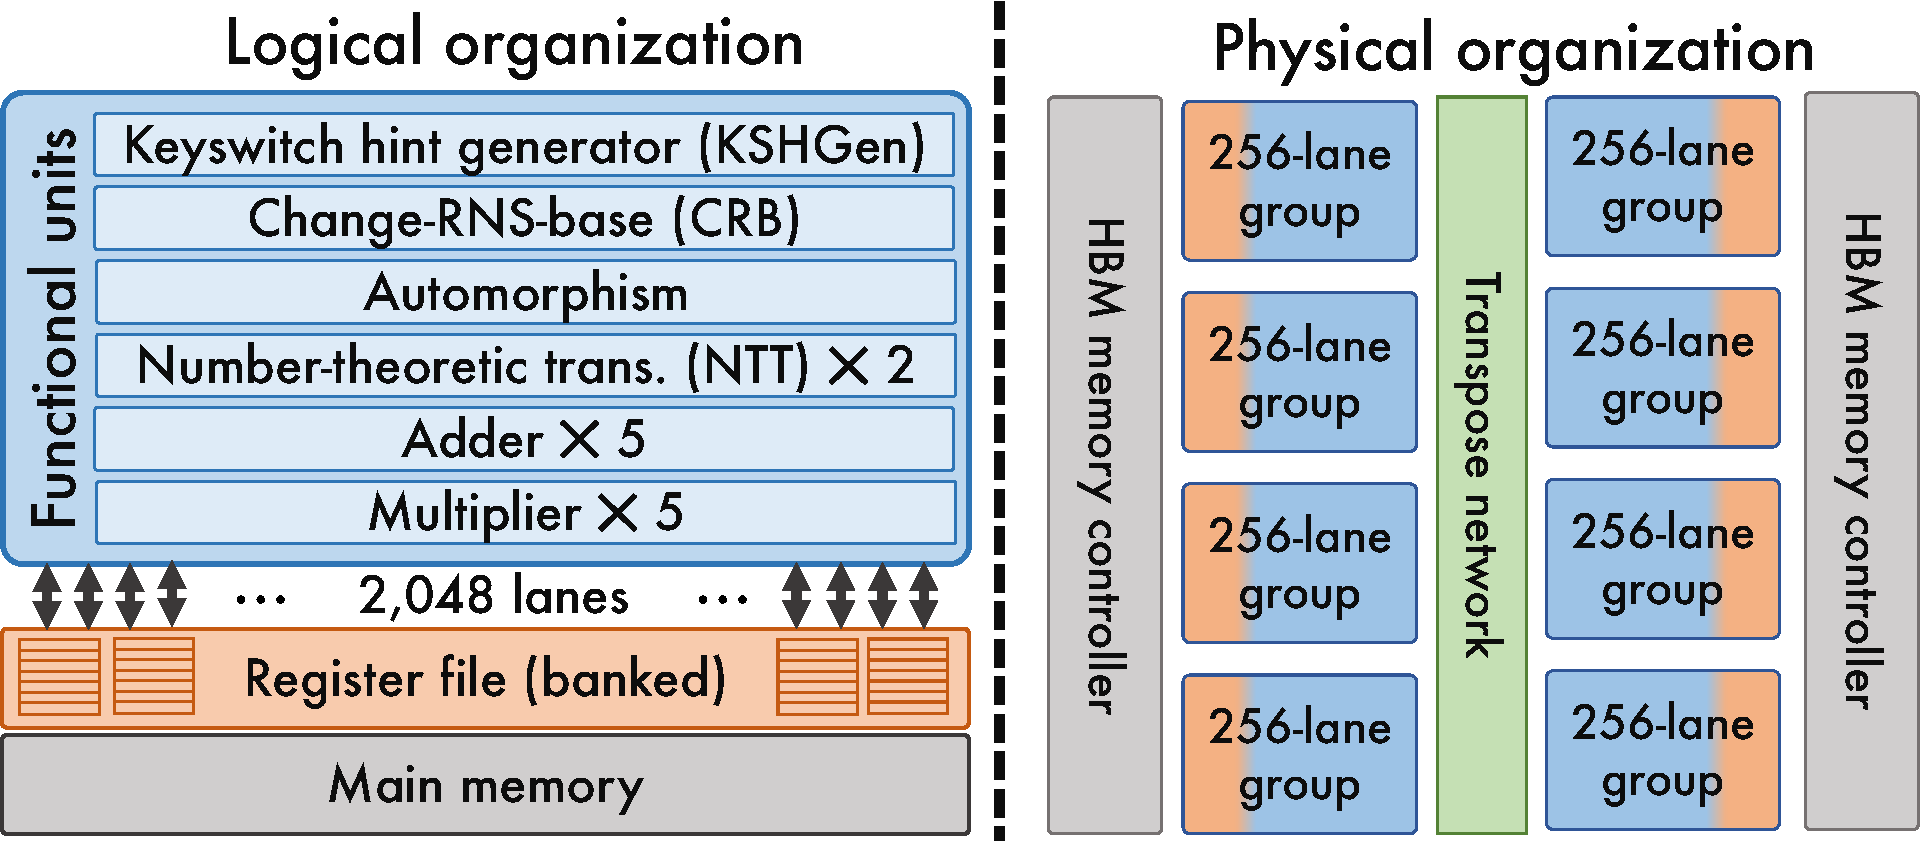
\includegraphics[width=0.7\columnwidth]{plots/overview.pdf}
        \caption{Overview of the \name architecture.}
        \label{fig:overview}
    \end{center}
  \end{figure}
}

\begin{comment}
\newcommand{\figTilingExample}{
    \begin{figure}[t]
        \begin{center}
            \includegraphics[width=\columnwidth]{figures/ag_tilingExample.pdf}
            \caption{Dividing the \emph{coeffToSlot} dataflow into partitions that fit on chip.}
            \label{fig:tilingExample}
        \end{center}
    \end{figure}
}
\end{comment}

\newcommand{\figTiling}{
  \begin{figure}[t]
    \begin{center}
        \includegraphics[width=\columnwidth]{figures/ag_tiling.pdf}
        \caption{Breakdown of different components of a ciphertext.}
        \label{fig:tiling}
    \end{center}
  \end{figure}
}

\newcommand{\tblBenchmarks}{
    \begin{table}[t]
        \begin{normalsize}
        \begin{center}
                \begin{tabular}{lrrrrr}
                    \toprule
                    Execution time (ms) on  & \name  & F1+   & CPU      & vs. F1+ & vs. CPU \\
                    \midrule
                    ResNet-20               & 249.45 & 2,693 & 23\,min &         10.8\x &          5,519\x \\
                    Logistic Regression     & 119.52 &   639 &  356\,s &         5.34\x &          2,978\x \\
                    LSTM                    & 138.00 & 2,573 &  859\,s &         18.6\x &          6,225\x \\
                    Packed Bootstrapping    &   3.91 &  58.3 & 17.2\,s &         14.9\x &          4,398\x \\
                    \midrule
                    \textbf{deep gmean speedup}  &&&                   & \textbf{11.2\x} & \textbf{4,611\x} \\
                    \midrule
                    Unpacked bootstrapping  &  0.10  & 0.21    &    877 &         2.04\x &          8,612\x \\
                    CIFAR Unencryp. Wghts.  & 50.50  & 94.1    & 187\,s &         1.86\x &          3,695\x \\
                    MNIST Unencryp. Wghts.  &  0.14  & 0.13    &    561 &         0.97\x &          4,152\x \\
                    MNIST Encryp. Wghts.    &  0.24  & 0.22    &   1369 &         0.88\x &          5,621\x \\
                    \midrule
                    \textbf{shallow gmean speedup} &&&                  &\textbf{1.34\x} & \textbf{5,220\x}  \\
                    \bottomrule
               \end{tabular}
       \end{center}
       \caption{Performance of \name, F1+, and CPU on full FHE benchmarks.}
       \label{tbl:benchmarks}
    \end{normalsize}
    \end{table}
}

\newcommand{\tblSecureBenchmarks}{
    \begin{table}[t]
        \begin{center}
            \begin{footnotesize}
                \begin{tabular}{lrr|rr}
                    \toprule
                    Execution time (ms) for & 128-bit  & vs. 80-bit & 200-bit ($N$=128k) & vs. 80-bit \\
                    \midrule
                    ResNet-20               & 321.26   & 1.29\x & 588.70 & 2.36\x \\
                    Logistic Regression     & 121.91   & 1.02\x & 123.10 & 1.03\x \\
                    LSTM                    & 223.56   & 1.62\x & 596.16 & 4.32\x \\
                    Packed Bootstrapping    &   6.33   & 1.62\x &  17.01 & 4.35\x \\
                    \midrule
                    \textbf{gmean slowdown}  && \textbf{1.36\x} & & \textbf{2.60\x} \\
                    \bottomrule
               \end{tabular}
            \caption{Performance of \name at 128-bit security and at 200-bit ($N$=128k) with comparisons to performance at 80-bit security.}
           \label{tbl:securebenchmarks}
            \end{footnotesize}
       \end{center}
    \end{table}
}

\newcommand{\figGmeanVsStorage}{
    \begin{figure}
            \centering
            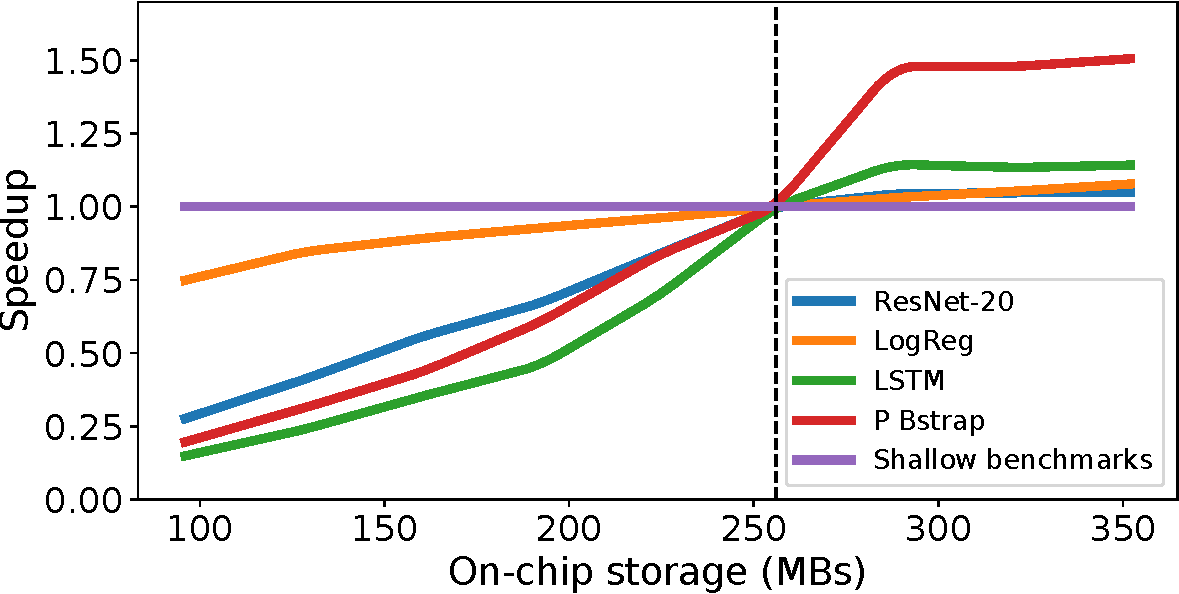
\includegraphics[width=0.65\columnwidth]{plots/scratchpad_sweep.pdf}
            \caption{Gmean performance of \name on deep benchmarks as a function of on-chip storage size.}
            \label{fig:gmeanVsStorage}
    \end{figure}
}

\newcommand{\tblPerformanceBreakdown}{
    \begin{table}[t]
        \begin{normalsize}
        \begin{center}
            \begin{tabular}{lrrrr}
                \toprule
                Speedup vs.             & KSHGen & CRB/chain & Network \\
                \midrule
                ResNet-20               & 2.0\x    & 20.0\x  & 1.7\x \\
                Logistic Regression     & 1.3\x    &  8.8\x  & 1.2\x \\
                LSTM                    & 2.5\x    & 34.5\x  & 1.3\x \\
                Packed Bootstrapping    & 2.0\x    & 27.4\x  & 1.3\x \\
                \midrule
                \textbf{deep gmean speedup} & \textbf{1.9\x} & \textbf{20.2\x} & \textbf{1.3\x} \\
                \midrule
                Unpacked Bootstrapping  &1.9\x & 3.7\x       & 1.0\x \\
                CIFAR Unencrypt. Wghts. &1.0\x & 3.7\x       & 2.0\x \\
                MNIST Unencrypt. Wghts. &1.1\x & 1.3\x       & 1.5\x \\
                MNIST Encryp. Wghts.    &1.1\x & 1.0\x       & 1.3\x \\
                \midrule
                \textbf{shallow gmean speedup}  &\textbf{1.2\x}    &\textbf{2.0\x} & \textbf{1.4\x} \\
                \bottomrule
            \end{tabular}
            \caption{Speedups of CraterLake over configurations without KSHGen, CRB or chaining, and the fixed network.}
            \label{tbl:performanceBreakdown}
        \end{center}
        \end{normalsize}
    \end{table}
}

\newcommand{\tblBenchmarksAndPerformanceBreakdown}{
    \tblBenchmarks
    \tblPerformanceBreakdown
}



\newcommand{\figDataMovementAndPower}{
    \begin{figure}[t]
        \begin{center}
            \captionsetup[subfigure]{labelformat=empty}
            \begin{subfigure}[b]{0.4\columnwidth}
                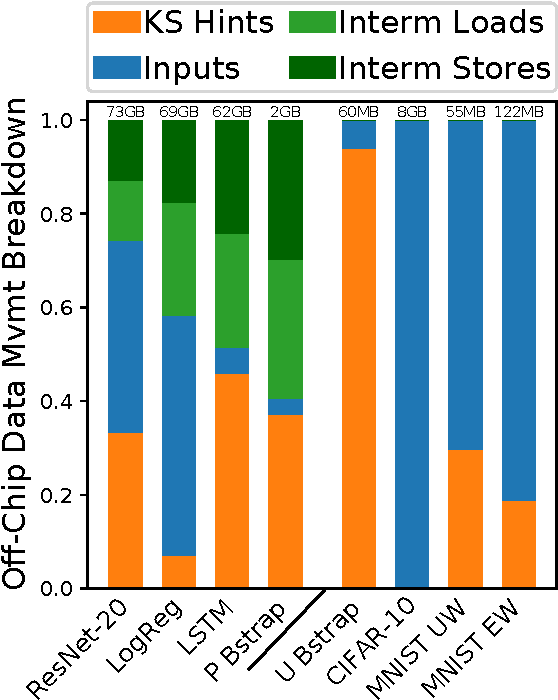
\includegraphics[width=\linewidth]{plots/cl_data_movement.pdf}
                \caption{}
                \label{fig:dataMovement}
            \end{subfigure}
            \hfil %%
            \begin{subfigure}[b]{0.4\columnwidth}
                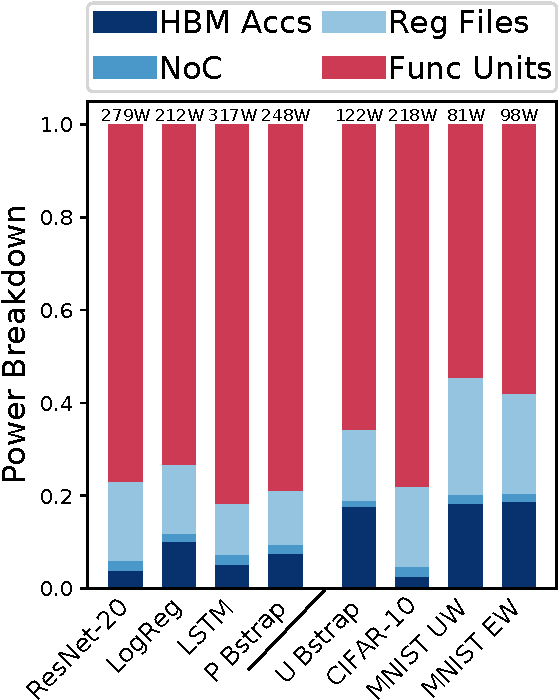
\includegraphics[width=\linewidth]{plots/cl_power.pdf}
                \caption{}
                \label{fig:power}
            \end{subfigure}
            \begin{center}
                (a) \hspace{0.47\columnwidth} (b)
            \end{center}
            \caption{Per-benchmark breakdown of (a) data movement and (b) average power for \name.}
        \end{center}
    \end{figure}
}

\newcommand{\tblMicrobenchmarks}{
    \begin{table}[t]
        \begin{footnotesize}
            \begin{center}
                \begin{tabular}{l|rr|rr|rr}
                    \toprule
                    & \multicolumn{2}{c|}{$N$=64K} & \multicolumn{2}{c|}{$N$=32K} & \multicolumn{2}{c}{$N$=16K} \\
                    Operation        & Ours  & vs. F1+ & Ours  & vs. F1+ & Ours & vs. F1+ \\
                    \midrule
                    Ct. mult.        & 8,436 & 6.13\x  & 2,260 & 3.00\x  &  708 & 1.31\x \\
                    Ct. rotate       & 6,388 & 7.85\x  & 1,748 & 3.66\x  &  580 & 1.43\x \\
                    Pt. rotate       & 4,096 & 0.25\x  & 1,024 & 0.25\x  &  256 & 0.25\x \\
                    Ct. add          & 1,024 & 0.25\x  &   256 & 0.25\x  &   64 & 0.25\x \\
                    Pt.-Ct. mult.    & 1,024 & 0.25\x  &   256 & 0.25\x  &   64 & 0.25\x \\
                    \bottomrule
                \end{tabular}
            \end{center}
            \caption{Performance of \name vs. F1+ on ciphertext operations. We report results in reciprocal throughput, in nanoseconds per ciphertext operation (lower is better). The benchmarks are in order: $(N, \log Q) = (64K, 1,664), (32K, 832), (16K, 416)$.}
            \label{tbl:microbenchmarks}
        \end{footnotesize}
    \end{table}
}

\newcommand{\tblDataTypes}{
    \begin{table}[t]
        \begin{center}
            \begin{tabular}{lrrr}
                \toprule
                Data type & Size vs. Pt & $L=10$ & $L=32$ \\
                \midrule
                Old Keyswitch Hint & $2L$\x & $20\,$MB & $208\,$MB \\
                New Keyswitch Hint & $4$\x & $4\,$MB & $12\,$MB \\
                Ciphertext & $2$\x & $2\,$MB & $6\,$MB \\
                Plaintext & $1$\x & $1\,$MB & $3\,$MB \\
                \bottomrule
            \end{tabular}
        \end{center}
        \caption{Comparison of sizes of different data types used in FHE.}
    \end{table}
}

\newcommand{\tblOpCost}{
    \begin{table}[t]\label{tbl:opCost}
        \begin{center}
            \begin{tabular}{lrrr}
                \toprule
                Operation & Integer mults & \% KS & \% total ops \\
                \midrule
                Ct-ct multiplication &$3 \times 10^{12}$ & $99.99\%$ & ??? \\
                Ct rotation &$3 \times 10^{12}$ & $100.00\%$ & ??? \\
                Pt-ct multiplication & $10^6$ & - & ??? \\
                Ct-ct addition &0 & - & ??? \\
                Pt-ct addition &0 & - & ??? \\
                Pt rotation &0 & - & ??? \\
                \bottomrule
            \end{tabular}
        \end{center}
        \caption{Computational cost of FHE operations.}
    \end{table}
}

\newcommand{\tblGF}{
  \begin{table}[t]
    \begin{center}
      \begin{normalsize}
        \begin{tabular}{lr}
          \toprule
    Component                                           & Area [mm$^2$] \\
    \midrule
    CRB FU                                              & 158.8 \\
    NTT FU                                              &  28.1 \\
    Automorphism FU                                     &   9.0 \\
    KSHGen FU                                           &   3.3 \\
    Multiply FU                                         &   2.2 \\
    Add FU                                              &   0.8 \\
    \mbox{\textbf{Total FUs} (CRB, 2$\times$NTT,}  & \textbf{240.5} \\
    \mbox{\hspace{2pt} Aut, KSHGen, 5$\times$Mul, 5$\times$Add)} & \\
    \midrule
    \mbox{Register file (256\,MB)}                      & 192.0 \\
    \mbox{On-chip interconnect}                         &  10.0 \\
    \mbox{Mem. PHYs (2$\times$HBM2E)}                   &  29.8 \\
    \midrule
    \textbf{Total \name}                                &  \textbf{472.3} \\
    \bottomrule
\end{tabular}
\end{normalsize}
\caption{Area breakdown of \name by component.}
\label{tbl:GF12}
\end{center}
\end{table}
}
